\section{Theorie}
\label{sec:Theorie}

\subsection{Einleitung}

Innerhalb dieses Experiments wird die Funktionsweise eines Helium-Neon Lasers untersucht.


\subsection{Funktionsweise eines Lasers}

Die wesentliche Eigenschaft eines Lasers ist, dass er mit Hilfe von stimulierter
Emission in der Lage ist, monochromatisches Licht mit hoher Intensität und
hoher Kohärenz also gleicher Phase zu erzeugen.
Um einen Laser zu realisieren werden im Allgemeinen drei Komponenten benötigt:
eine Pumpquelle, ein Lasermedium und einen Resonator. Im Lasermedium muss durch die zugeführte
Energie der Pumpquelle eine Besetzungsinversion induziert werden können
damit der Laser überhaupt funktionieren kann. Um dies genauer zu erläutern,
werden im folgenden Abschitt zunächst verschiedene Arten von Emission und Absorption
anhand eines Zweiniveausystems erklärt.

Im thermodynamischen Gleichgewicht und ohne äußere Energiezufuhr ist der Grundzustand im
Zweiniveausystem stärker besetzt als der angeregte Zustand. Pumpt man Photonen mit einer Energie,
die der Energiedifferenz der beiden Niveaus entspricht, in das System, so werden diese mit der Rate
\begin{align}
  \frac{\mathrm{d}{N}_A}{\mathrm{d}t} = n_1 \rho(\nu) B_{12}
\end{align}
absorbiert, wobei ein Elektron vom Grundzustand in den angeregten Zustand angehoben wird. Dabei ist $n_1$
die Besetzungszahl des Grundzustands, $\rho(\nu)$ das Strahlungsfeld und $B_{12}$ ein sogenannter
Einsteinkoeffizient. Andersherum kann ein Elektron auch unter Emission eines Photons vom angeregten
Zustand in den Grundzustand übergehen. Dabei wird zwischen spontaner Emission, die unabhängig vom
externen Strahlungsfeld auftritt gemäß der Rate
\begin{align}
  \frac{\mathrm{d}{N}_\text{spont}}{\mathrm{d}t} = n_2 A_{21},
\end{align}
und induzierter Emission, deren Rate
\begin{align}
  \frac{\mathrm{d}{N}_\text{ind}}{\mathrm{d}t} = n_2 \rho(\nu) B_{21}
\end{align}
proportional zum Strahlungsfeld ist, unterschieden. Alle drei beschriebenen Fälle sind in Abbildung
\ref{fig:absemi} skizziert.

\begin{figure}
  \centering
  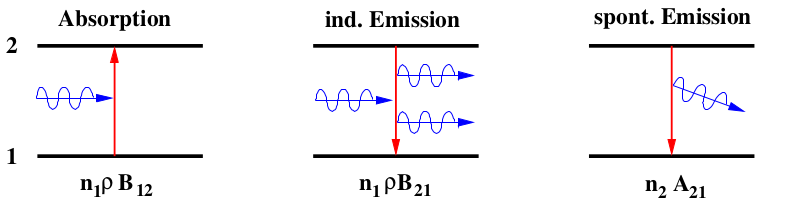
\includegraphics[height = 6cm]{Pics von Buddy/absemi.png}
  \caption{\cite{anleitung}.}
  \label{fig:absemi}
\end{figure}


\cite{anleitung}
